\section{Why dependence-based rules do not lead: mechanisms}\label{sec:mech}

Sections~\ref{sec:coll}--\ref{sec:subsets} say that the benchmarks are small and that no rule leads across them. They do not say why the rules that test the conditional structure of the pair do not do better. We tested three explanations, each with a prediction fixed before the run (experiments 49--52, 56, 57), and report the ones that failed.

\subsection{The benchmarks can be solved from the marginals}\label{sec:marg}
\emph{Hypothesis.} On the real collections, a classifier that never sees the joint distribution of $(x,y)$, only the two marginal distributions, orients the pairs about as well as the best rule. If so, the benchmark rewards a rule's sensitivity to marginal asymmetry between cause and effect, a property that conditional-structure rules do not use.

\emph{Classifier.} Each variable is scaled to $[0,1]$ and described by five numbers: skewness, excess kurtosis, Vasicek spacing entropy ($m=\sqrt n$), the logarithm of the fraction of unique values, and the $1$--$99\%$ range. The pair feature is the difference of the two vectors; both orientations enter training with labels $1$ and $0$; the model is a standardised logistic regression. The first protocol (experiment 49) uses five-fold cross-validation with folds over pairs ($50$ repetitions): $59.0\%$ on T\"ubingen, $100\%$ on the i.i.d.\ chamber pairs, $92.6\%$ on the walk pairs and $89.8\%$ on the Sachs pairs.

\emph{These first numbers leak.} The chamber edges share their cause variable (\texttt{load\_in} causes many sensors) and the 17 Sachs arcs reuse eleven proteins, so a held-out pair often had its variable's marginal in the training folds. Review of the first version identified the problem; experiment 52 removes it:
\begin{itemize}
\item i.i.d.\ chambers: training on the wind-tunnel recording and testing on the light-tunnel recording and conversely, $97.9\%$ ($93.6\%$ without the unique-fraction feature);
\item walk recordings: leaving one of the five recordings out, $86.9\%$ ($90.2\%$) (recordings of the same tunnel share variable names, so this is a weaker test than the wind-to-light transfer above, which is cross-device);
\item Sachs: training on the arcs that involve neither protein of the test arc, $94.1\%$ (all $17$ arcs evaluated; same with or without the feature);
\item T\"ubingen: leave one pair out, $57.8\%$.
\end{itemize}
The unique-fraction feature separates discrete actuators from continuous sensors and is a measurement artefact when sets are preprocessed differently (T\"ubingen is dequantised, so the feature is constant there); dropping it leaves the picture unchanged. The prediction held: above $80\%$ without leakage.

\begin{figure}[t]
\centering
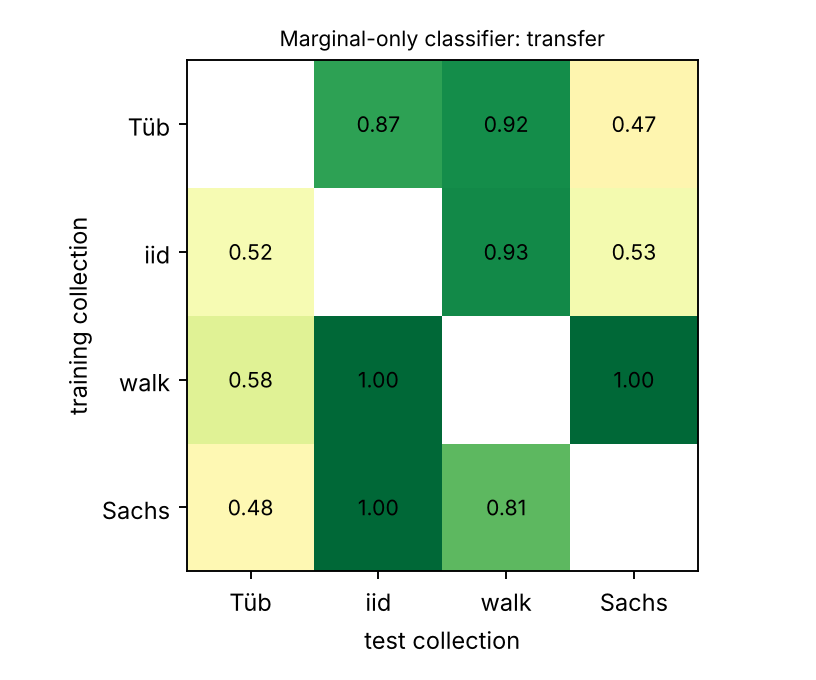
\includegraphics[width=0.55\linewidth]{figs/transfer.png}
\caption{Marginal-only classifier trained on one collection (rows) and tested on another (columns), accuracy. The cue learned on T\"ubingen, Sachs or the chambers orients the chamber pairs; nothing learned on the chambers or Sachs transfers to T\"ubingen.}
\label{fig:transfer}
\end{figure}

\emph{Transfer across collections.} A classifier trained on the $102$ T\"ubingen pairs orients $87.2\%$ of the i.i.d.\ chamber pairs and $91.8\%$ of the walk pairs; one trained on the $17$ Sachs pairs orients $100\%$ of the i.i.d.\ chamber pairs ($96.8\%$ without the unique-fraction feature) and $81.1\%$ of the walk pairs; one trained on the chambers does not orient T\"ubingen ($52\%$ for the i.i.d.-trained and $58\%$ for the walk-trained model); Sachs is oriented by the walk-trained model ($100\%$, $88\%$ without the unique-fraction feature) but not by the i.i.d.-trained one ($53\%$; the Sachs set has $17$ pairs). Figure~\ref{fig:transfer} shows the matrix. The marginal asymmetry between an experimenter-set actuator and a sensor is a property shared by every device, and it is not present in T\"ubingen in a way that transfers: on T\"ubingen the marginal-only accuracy ($57.8$--$59.0\%$) is within the sampling error of chance and of most dependence-based rules.

\emph{What this does and does not show.} It does not show that RECI or IGCI use only the marginals: both read the scale of regression errors and the marginal density. It shows that the chamber collections can be oriented from the marginals alone, so a rule that is sensitive to marginal asymmetry will do well on them for reasons that have nothing to do with conditional structure, and that a rule that tests only the conditional model, such as an additive-noise test, has no reason to profit. That the chamber rankings (Figure~\ref{fig:collections}) look like the marginal cue and the T\"ubingen ranking does not is consistent with this and is the first leg of the explanation.

\subsection{Additive-noise rules work in one regime and reverse in another}\label{sec:regimes}
\emph{Hypothesis.} The additive-noise family loses where its assumption fails. For every T\"ubingen pair we measured the heteroscedasticity of the residuals of a cross-fitted additive-spline regression of the true effect on the true cause: $h=|\rho_S(|r|,x)|$ with $\rho_S$ the Spearman correlation (six knots, ridge penalty one, two folds). Table~\ref{tab:h2} gives, for each rule, the mean $h$ on the pairs it orients wrongly and rightly. The four noise-model rules show a large difference: ANM-HSIC $0.32$ against $0.13$, the Gaussian-process ANM $0.29$ against $0.10$, RESIT $0.34$ against $0.13$, LOCI $0.27$ against $0.17$ (one-sided Mann--Whitney, $p\le 0.0014$ for each); also TRA ($p=0.004$) and, weakly, RECI ($p=0.021$) and PDM ($p=0.021$); not IGCI ($p=0.71$), pairwise LiNGAM ($p=0.25$), AVICI ($p=0.93$) or the compression rules ($p=0.075$ to $0.095$). Pooling the decisions of the four noise-model rules ($396$ decisions) in a logistic regression of correctness on the standardised $h$ and $\log n$, one standard deviation of $h$ multiplies the odds of a correct decision by $0.26$ ($p<10^{-18}$, optimistic because the four rules are scored on the same pairs); $n$ has no effect ($p=0.94$). We had predicted that RECI would not show the effect; it does, mildly.

\begin{table}[t]
\caption{T\"ubingen: mean residual heteroscedasticity $h$ (true direction) on the pairs a rule orients wrongly and rightly; $p$: one-sided Mann--Whitney test that $h$ is larger on the wrong pairs. Twelve rules, no multiplicity correction.}
\label{tab:h2}
\small
\begin{tabular}{@{}lcccc@{}}
\toprule
Rule & wrong/right & $h$ wrong & $h$ right & $p$\\
\midrule
IGCI & 45/57 & 0.19 & 0.22 & 0.707\\
RECI & 40/62 & 0.25 & 0.17 & 0.021\\
ANM-HSIC & 40/62 & 0.32 & 0.13 & 0.000\\
Pairwise LiNGAM & 40/62 & 0.22 & 0.19 & 0.245\\
PDM & 61/41 & 0.22 & 0.18 & 0.021\\
LOCI & 36/66 & 0.27 & 0.17 & 0.001\\
ANM, Gaussian process & 42/53 & 0.29 & 0.10 & 0.000\\
Compression, first impl. & 40/62 & 0.22 & 0.19 & 0.088\\
Compression, first impl., raw & 36/66 & 0.22 & 0.19 & 0.095\\
TRA & 29/53 & 0.26 & 0.17 & 0.004\\
Compression, faithful & 34/68 & 0.23 & 0.19 & 0.075\\
AVICI & 42/60 & 0.18 & 0.22 & 0.926\\
RESIT & 37/60 & 0.34 & 0.13 & 0.000\\
\bottomrule
\end{tabular}
\end{table}

Splitting T\"ubingen into thirds by $h$ (bounds $0.094$ and $0.268$, $34$ pairs each; TRA has $24$, $31$ and $27$ pairs with a value) shows the regimes (Table~\ref{tab:strata}, Figure~\ref{fig:strata}). In the least heteroscedastic third ANM-HSIC, RESIT and the Gaussian-process ANM are right on $97\%$, $96\%$ and $91\%$ of the pairs, far above RECI ($68\%$); in the most heteroscedastic third on $29\%$, $24\%$ and $22\%$, below chance. Averaged over the three thirds, ANM-HSIC ($0.61$) and RESIT ($0.62$) equal the baselines and the Gaussian-process ANM is lower ($0.55$): a rule that is excellent in one regime and reversed in another has the accuracy of one that is mediocre in both. This reading is descriptive: $h$ is computed in the true direction, so it is not a predictor; its bounds come from the same data; it is close to the dependence between the scale and the cause that the additive-noise tests probe, so part of the association is by construction.

\begin{table}[t]
\caption{T\"ubingen accuracy by tercile of $h$ ($34$ pairs per tercile; TRA $24$, $31$, $27$).}
\label{tab:strata}
\small
\begin{tabular}{@{}lccc@{}}
\toprule
Rule & low $h$ & middle & high $h$\\
\midrule
ANM-HSIC & 0.97 & 0.56 & 0.29\\
RESIT & 0.96 & 0.65 & 0.24\\
ANM, Gaussian process & 0.91 & 0.53 & 0.22\\
TRA & 0.83 & 0.68 & 0.44\\
LOCI & 0.82 & 0.62 & 0.50\\
RECI & 0.68 & 0.68 & 0.47\\
IGCI & 0.59 & 0.44 & 0.65\\
Pairwise LiNGAM & 0.65 & 0.53 & 0.65\\
Compression, faithful & 0.74 & 0.74 & 0.53\\
Compression, first impl., raw & 0.71 & 0.68 & 0.56\\
AVICI & 0.53 & 0.56 & 0.68\\
PDM & 0.56 & 0.35 & 0.29\\
\bottomrule
\end{tabular}
\end{table}

\begin{figure}[t]
\centering
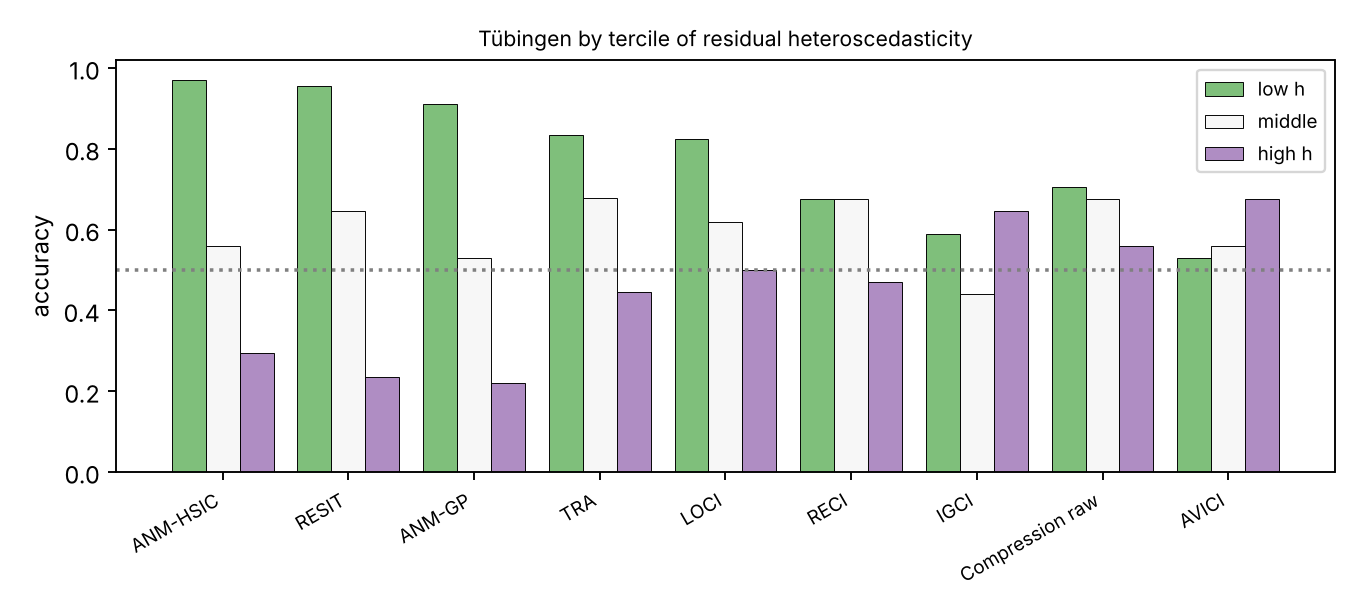
\includegraphics[width=0.85\linewidth]{figs/strata.png}
\caption{T\"ubingen accuracy by tercile of the residual heteroscedasticity $h$.}
\label{fig:strata}
\end{figure}

\subsection{Manipulation with a marginal control}\label{sec:dose}
An association across pairs cannot separate heteroscedasticity from whatever else differs between pairs, and making the noise scale depend on the cause also changes the marginal of the effect (a scale mixture). We therefore set the factor by hand (experiment 52). Pairs $e=f(c)+\sigma\varepsilon$, $f\in\{\tanh 2c,c^3/3,\sin 1.5c\}$, $c$ uniform or Gaussian, $n=500$, the same $c$, $f$ and $\varepsilon$ at every level, $a\in\{0,0.5,1,1.5\}$, $100$ pairs per level, a random half swapped. In the heteroscedastic arm $\sigma(c)\propto\exp(ac)$; in the control arm $\sigma_i\propto\exp(au_i)$ with $u_i\sim N(0,1)$ independent of $c$, which gives the effect a similar heavy-tailed marginal but no dependence of the scale on the cause; the average noise variance is fixed in both. Figure~\ref{fig:dose} and Table~\ref{tab:dose}: ANM-HSIC falls from $100\%$ to $21\%$ with cause-dependent noise and only to $89\%$ with the independent scale, so the collapse is due to the dependence of the scale on the cause. IGCI and RECI rise in both arms ($64\to99\%$ and $78\to93\%$ with cause-dependent noise; $64\to99\%$ and $78\to98\%$ with the independent scale): they profit from the heavy-tailed marginal of the effect, not from heteroscedasticity. An earlier unmatched run without the control showed the same rise and we had attributed it to heteroscedasticity; the control refutes that, and the correct reading ties this experiment to Section~\ref{sec:marg}: IGCI and RECI are sensitive to marginal asymmetry.

\begin{table}[t]
\caption{Matched simulated pairs: accuracy against the strength $a$ ($100$ pairs per level). Left: noise scale depends on the cause. Right: independent random scale with the same kind of marginal (control).}
\label{tab:dose}
\small
\begin{tabular}{@{}lcccc|cccc@{}}
\toprule
 & \multicolumn{4}{c|}{scale depends on cause} & \multicolumn{4}{c}{independent scale}\\
Rule & $0$ & $0.5$ & $1$ & $1.5$ & $0$ & $0.5$ & $1$ & $1.5$\\
\midrule
ANM-HSIC & 1.00 & 0.49 & 0.12 & 0.21 & 1.00 & 1.00 & 0.99 & 0.89\\
IGCI & 0.64 & 0.72 & 0.91 & 0.99 & 0.64 & 0.73 & 0.95 & 0.99\\
RECI & 0.78 & 0.77 & 0.87 & 0.93 & 0.78 & 0.84 & 0.96 & 0.98\\
\bottomrule
\end{tabular}
\end{table}

\begin{figure}[t]
\centering
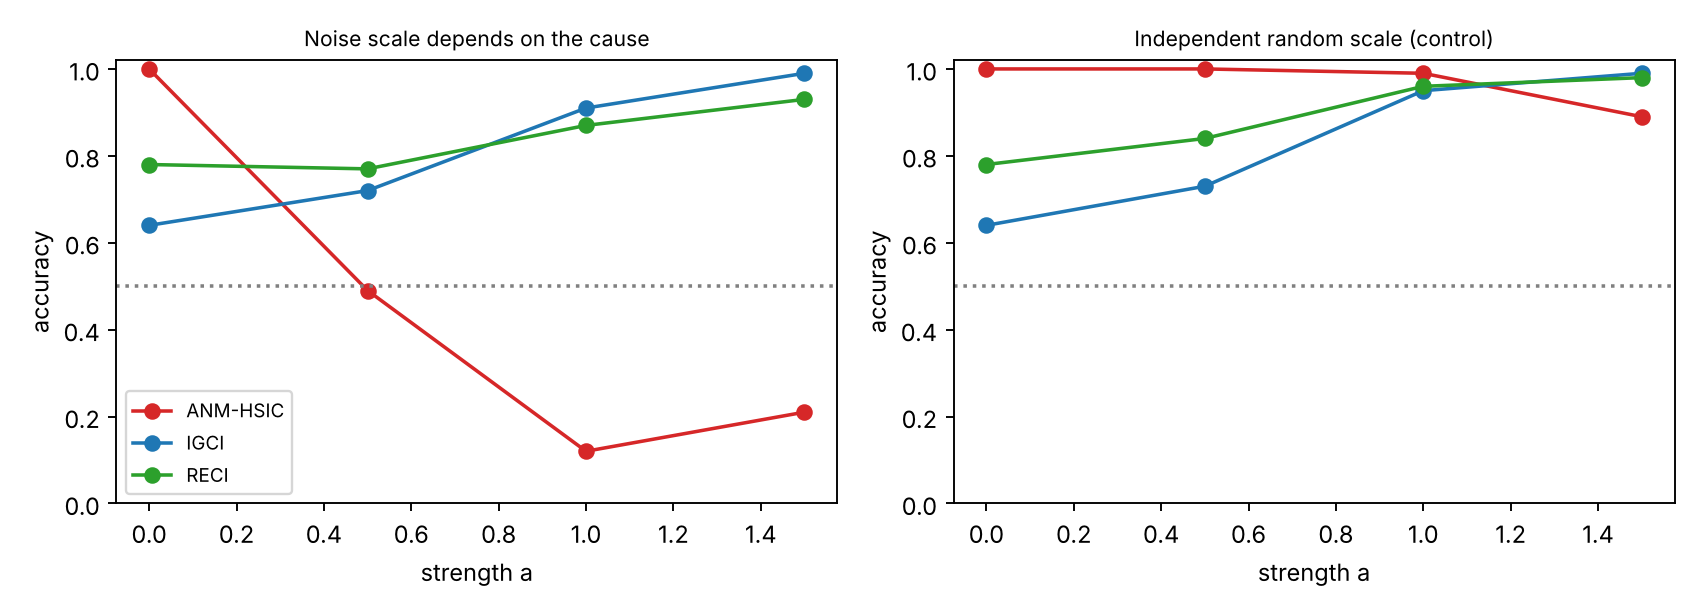
\includegraphics[width=0.95\linewidth]{figs/dose.png}
\caption{Accuracy against the strength $a$ of the noise-scale variation. Left: scale depends on the cause. Right: independent scale (control).}
\label{fig:dose}
\end{figure}

\subsection{A factorial map}\label{sec:factorial}
To see the regimes together we crossed five factors (experiment 56): the mechanism ($\tanh 2c$, $c^3/3$, $\sin 1.5c$), the cause marginal (uniform, normal, bimodal, five-level discrete), the noise scale (homoscedastic, cause-dependent, independent random), measurement noise on both variables ($0$ or $0.3$ sd), and $n\in\{200,1000\}$: $144$ cells of $25$ pairs ($3600$ pairs), seven rules. Table~\ref{tab:factorial} gives the accuracy by factor level and Table~\ref{tab:factorial2} the interaction of the noise scale with measurement noise.

\begin{table}[t]
\caption{Factorial simulation (3600 pairs): accuracy of seven rules averaged over the other factors.}
\label{tab:factorial}
\small
\setlength{\tabcolsep}{3pt}
\begin{tabular}{@{}llccccccc@{}}
\toprule
Factor & Level & IGCI & RECI & ANM-HSIC & LiNGAM & Compr. & RESIT & AVICI\\
\midrule
mechanism & tanh & 0.66 & 0.71 & 0.42 & 0.16 & 0.65 & 0.46 & 0.66\\
mechanism & cubic & 0.87 & 1.00 & 0.70 & 0.54 & 0.75 & 0.75 & 0.19\\
mechanism & sin & 0.55 & 0.95 & 0.73 & 0.81 & 0.74 & 0.75 & 0.85\\
cause marginal & uniform & 0.94 & 0.95 & 0.52 & 0.34 & 0.84 & 0.53 & 0.49\\
cause marginal & normal & 0.61 & 0.72 & 0.64 & 0.36 & 0.84 & 0.68 & 0.89\\
cause marginal & bimodal & 0.75 & 0.89 & 0.63 & 0.59 & 0.79 & 0.68 & 0.36\\
cause marginal & discrete5 & 0.47 & 0.97 & 0.68 & 0.71 & 0.39 & 0.72 & 0.53\\
noise scale & homoscedastic & 0.56 & 0.82 & 0.82 & 0.50 & 0.68 & 0.84 & 0.55\\
noise scale & cause & 0.74 & 0.90 & 0.28 & 0.56 & 0.72 & 0.36 & 0.66\\
noise scale & independent scale & 0.78 & 0.94 & 0.75 & 0.45 & 0.74 & 0.76 & 0.49\\
measurement noise & 0 & 0.61 & 0.92 & 0.64 & 0.50 & 0.70 & 0.67 & 0.58\\
measurement noise & 1 & 0.77 & 0.85 & 0.59 & 0.50 & 0.73 & 0.64 & 0.56\\
n & 200 & 0.66 & 0.87 & 0.61 & 0.52 & 0.62 & 0.66 & 0.58\\
n & 1000 & 0.73 & 0.90 & 0.62 & 0.48 & 0.81 & 0.65 & 0.55\\
\bottomrule
\end{tabular}
\end{table}

\begin{table}[t]
\caption{Factorial simulation: noise scale $\times$ measurement noise.}
\label{tab:factorial2}
\small
\setlength{\tabcolsep}{3pt}
\begin{tabular}{@{}llccccccc@{}}
\toprule
Noise scale & Meas. noise & IGCI & RECI & ANM-HSIC & LiNGAM & Compr. & RESIT & AVICI\\
\midrule
homoscedastic & no & 0.47 & 0.89 & 0.95 & 0.49 & 0.67 & 0.95 & 0.54\\
homoscedastic & yes & 0.64 & 0.76 & 0.69 & 0.50 & 0.69 & 0.74 & 0.55\\
cause-dependent & no & 0.68 & 0.91 & 0.06 & 0.55 & 0.71 & 0.17 & 0.68\\
cause-dependent & yes & 0.81 & 0.89 & 0.49 & 0.56 & 0.73 & 0.54 & 0.65\\
independent scale & no & 0.69 & 0.98 & 0.91 & 0.46 & 0.70 & 0.89 & 0.52\\
independent scale & yes & 0.86 & 0.90 & 0.60 & 0.45 & 0.78 & 0.64 & 0.47\\
\bottomrule
\end{tabular}
\end{table}

The additive-noise rules are near-perfect only in the cell with homoscedastic noise and no measurement noise (ANM-HSIC $0.95$, RESIT $0.95$), fall to $0.69$ and $0.74$ with measurement noise alone, and to $0.06$ and $0.17$ with a cause-dependent scale; measurement noise partly masks the reversal ($0.49$, $0.54$). IGCI and the faithful compression are the weakest rules when the cause is discrete ($0.47$ and $0.39$); IGCI is more accurate with measurement noise than without ($0.77$ against $0.61$); the faithful compression depends on $n$ ($0.62$ at $200$, $0.81$ at $1000$); AVICI fails on the cubic mechanism ($0.19$) and is at $0.49$ for the uniform cause. RECI has the highest average accuracy in $12$ of the $14$ factor levels (the exceptions are the normal cause, where AVICI is at $0.89$ against $0.72$, and homoscedastic noise, where RESIT is at $0.84$ against $0.82$). Which factor breaks which rule is rule-specific.

\subsection{An assumption-gated rule fails}\label{sec:gate}
If the regimes explain the T\"ubingen average, a rule that identifies the regime should beat both of its branches. We froze GATE on simulation before touching a real pair (experiment 51): $h_{\min}=\min(h(x\to y),h(y\to x))$, symmetric in the variables, threshold at the $95$th percentile of $h_{\min}$ on $200$ homoscedastic simulated pairs ($0.058$ at $n=500$); GATE returns the ANM-HSIC direction when $h_{\min}\le 0.058$ and the RECI direction otherwise. The pre-registered predictions were an accuracy of at least $0.70$ on T\"ubingen and, on the chambers, within $0.05$ of RECI. Both failed. On T\"ubingen GATE has $65.7\%$ ($77.1\%$ with the official weights) against $60.8\%$ ($70.9\%$) for RECI; it routes $34\%$ of the pairs to ANM-HSIC and the difference to RECI is not significant (exact McNemar $10$ against $5$, $p=0.30$). On the i.i.d.\ chambers GATE has $75.5\%$ against $97.9\%$ ($0$ against $21$ discordant pairs, $p<10^{-6}$) and on the walks $77.0\%$ against $94.3\%$ ($p<10^{-6}$), because it sends $88\%$ and $62\%$ of those pairs to ANM-HSIC, which is right on $72\%$ and $63\%$ of the whole collections (we did not store its accuracy on the routed subset). The threshold was set at $n=500$, the chamber pairs have $n=2000$ and the null spread of $|\rho|$ shrinks with $n$, so the routing is not comparable across sets; an $n$-aware threshold was not tried. The Sachs pairs were not evaluated (no stored ANM-HSIC decision under the same preprocessing). GATE is a negative result and is not offered as a method.

\subsection{An attempt to predict real accuracy from the factorial map fails}\label{sec:predict}
The strongest test of an explanation is that it predicts. For every real pair we computed seven label-free diagnostics (minimum heteroscedasticity over the two directions, log fraction of unique values, minimum and maximum excess kurtosis, maximum absolute skewness, log absolute Spearman correlation, $\log n$), found its $100$ nearest neighbours among the $3600$ simulated pairs of Section~\ref{sec:factorial}, and predicted each rule's accuracy by the neighbours' mean correctness (experiment 57). The pre-registered criteria were a Spearman correlation of at least $0.5$ between predicted and observed accuracy over the $49$ (collection, rule) cells, a smaller RMSE than the constant prediction (each rule's overall simulation accuracy), and the rule predicted best being among the two best observed on at least four of the seven collections.

The first run was invalid as implemented: the unique-fraction diagnostic was constant in the simulation (computed on jittered arrays), so real pairs with tied values had standardised values around $-3\times10^{9}$ and the neighbours were arbitrary (Spearman $-0.01$). Revision 2 computes simulated and real diagnostics identically (the simulator is deterministic) and reports how far the real pairs are from the simulation. It fails as well: Spearman $0.17$ (criterion $0.5$), RMSE $0.30$ against $0.26$ for the constant prediction, and the predicted best rule is among the top two observed on $3$ of $7$ collections (this criterion is nearly degenerate: RECI is predicted best for every collection). The pair-level criterion, the AUC of the predicted correctness for the observed correctness, was also pre-registered and gives $0.67$ for RESIT, $0.63$ for ANM-HSIC and $0.44$ to $0.55$ for the five other rules, so the prediction carries some pair-level information for two of the seven rules and none for the others. The reason is visible in the support: the median distance from a real pair to its nearest simulated pair, in units of the simulation's standard deviations (a Euclidean metric on seven standardised diagnostics), is $2.3$ for T\"ubingen, $2.8$--$3.4$ for the chamber collections, $4.4$--$4.6$ for the Bernoulli and changepoint collections, $8.9$ for Sachs and $13.1$ for Malus, against a $95$th-percentile leave-one-out distance of $0.76$ within the simulation; at most $5\%$ of the pairs of any collection lie within the simulation's support. The factorial simulator illustrates mechanisms and cannot be used to predict accuracy on these real collections. The explanation of Sections~\ref{sec:marg}--\ref{sec:factorial} is therefore a set of demonstrated mechanisms, not a validated predictive model, and we do not claim that it accounts for the whole of the differences between the collections.

\subsection{Summary of the evidence on mechanisms}
Two mechanisms are directly supported. (1) The chamber and Sachs collections can be oriented from the marginals alone, validated across recordings and across proteins, and the same cue transfers across collections; IGCI and RECI are sensitive to marginal asymmetry and gain accuracy from a heavy-tailed effect marginal in simulation even when the conditional structure is unchanged. (2) Additive-noise rules are regime-specific: near-perfect when the noise scale does not depend on the cause and reversed when it does (manipulation with a control, factorial map, T\"ubingen terciles), and degraded by measurement noise. The T\"ubingen average of these rules equals the baselines because the collection mixes regimes. Two attempts to build on the account fail (GATE, predictive validation). What the evidence leaves unexplained is why the additive-noise rules lose on the chambers and how much of the differences between collections the two mechanisms jointly account for.
